%% Template for Stata-Journal Quarto manuscript

%% Main

% main.tex - a driver for your Stata Journal insert
% This file should only be changed according to the AUTHOR notes below.
% The Stata Press document class

\documentclass[bib]{statapress}

% Page dimensions
\usepackage[crop,newcenter,frame]{pagedims}
% The Stata Journal styles
\usepackage{sj}
% Stata Log listings and useful macros
\usepackage{stata}
% Encapsulated PostScript figures
\usepackage{epsfig}
% Shadow package to render technical note figure
\usepackage{shadow}
\usepackage{amsmath,amssymb} 
% EDITORS: volume number, issue number, month, and year
\usepackage{setspace}
%% Hide Links
%CodeThis is for Executed code. But may not be necessary
\usepackage{color}
\usepackage{fancyvrb}
\newcommand{\VerbBar}{|}
\newcommand{\VERB}{\Verb[commandchars=\\\{\}]}
\DefineVerbatimEnvironment{Highlighting}{Verbatim}{commandchars=\\\{\}}
% Add ',fontsize=\small' for more characters per line
\usepackage{framed}
\definecolor{shadecolor}{RGB}{255,255,255}
\newenvironment{Shaded}{\begin{snugshade}}{\end{snugshade}}
\newcommand{\KeywordTok}[1]{\textcolor[rgb]{0.00,0.0,0.0}{#1}}
\newcommand{\NormalTok}[1]{\textcolor[rgb]{0.00,0.0,0.0}{#1}}




%% Ref

 

\sjsetissue{vv}{ii}{mm}{yyyy}

%%%%%%%%%%%%%%%%%%%%%%%%%%%%%%%%%%%%%%%%%%%%%%%%%%%%%%%%%%%%%%%%%%%%%%%%%%%%%%%


\providecommand{\tightlist}{%
  \setlength{\itemsep}{0pt}\setlength{\parskip}{0pt}}\usepackage{longtable,booktabs,array}
\usepackage{calc} % for calculating minipage widths
% Correct order of tables after \paragraph or \subparagraph
\usepackage{etoolbox}
\makeatletter
\patchcmd\longtable{\par}{\if@noskipsec\mbox{}\fi\par}{}{}
\makeatother
% Allow footnotes in longtable head/foot
\IfFileExists{footnotehyper.sty}{\usepackage{footnotehyper}}{\usepackage{footnote}}
\makesavenoteenv{longtable}
\usepackage{graphicx}
\makeatletter
\newsavebox\pandoc@box
\newcommand*\pandocbounded[1]{% scales image to fit in text height/width
  \sbox\pandoc@box{#1}%
  \Gscale@div\@tempa{\textheight}{\dimexpr\ht\pandoc@box+\dp\pandoc@box\relax}%
  \Gscale@div\@tempb{\linewidth}{\wd\pandoc@box}%
  \ifdim\@tempb\p@<\@tempa\p@\let\@tempa\@tempb\fi% select the smaller of both
  \ifdim\@tempa\p@<\p@\scalebox{\@tempa}{\usebox\pandoc@box}%
  \else\usebox{\pandoc@box}%
  \fi%
}
% Set default figure placement to htbp
\def\fps@figure{htbp}
\makeatother

\makeatletter
\@ifpackageloaded{caption}{}{\usepackage{caption}}
\AtBeginDocument{%
\ifdefined\contentsname
  \renewcommand*\contentsname{Table of contents}
\else
  \newcommand\contentsname{Table of contents}
\fi
\ifdefined\listfigurename
  \renewcommand*\listfigurename{List of Figures}
\else
  \newcommand\listfigurename{List of Figures}
\fi
\ifdefined\listtablename
  \renewcommand*\listtablename{List of Tables}
\else
  \newcommand\listtablename{List of Tables}
\fi
\ifdefined\figurename
  \renewcommand*\figurename{Figure}
\else
  \newcommand\figurename{Figure}
\fi
\ifdefined\tablename
  \renewcommand*\tablename{Table}
\else
  \newcommand\tablename{Table}
\fi
}
\@ifpackageloaded{float}{}{\usepackage{float}}
\floatstyle{ruled}
\@ifundefined{c@chapter}{\newfloat{codelisting}{h}{lop}}{\newfloat{codelisting}{h}{lop}[chapter]}
\floatname{codelisting}{Listing}
\newcommand*\listoflistings{\listof{codelisting}{List of Listings}}
\makeatother
\makeatletter
\makeatother
\makeatletter
\@ifpackageloaded{caption}{}{\usepackage{caption}}
\@ifpackageloaded{subcaption}{}{\usepackage{subcaption}}
\makeatother
\begin{document}

%% AUTHOR:  Include your article here.

%% TITLE

 
\title[]{Simplifying the Estimation of Correlated Random Effects Models}


\makeatletter

\inserttype[st0001]{article}
\author{}{
Fernando Rios-Avila
\\
Universidad Privada Boliviana\\
La Paz, Bolivia\\

\href{mailto:f.rios.a@gmail.com}{f.rios.a@gmail.com}
}
 
 
 

\maketitle

\begin{abstract}

This paper introduces \texttt{cre}, a Stata prefix command designed to
simplify the implementation of Correlated Random Effects (CRE) models,
following the \citet{mundlak1978pooling} approach, for a wide range of
linear and nonlinear estimation commands. Standard Fixed Effects (FE)
estimators, while consistent under unobserved heterogeneity, cannot
identify coefficients for time-invariant variables. Standard Random
Effects (RE) estimators can identify such coefficients but rely on the
strong, often violated, assumption that individual effects are
uncorrelated with regressors. CRE models offer an empirical middle
ground, providing FE-equivalent estimates for time-varying coefficients
in linear models while still allowing identification of time-invariant
effects. The \texttt{cre} command facilitates this by automatically
generating the required group means of time-varying regressors and
adding them to the specified model, handling both balanced and
unbalanced panels. It also integrates seamlessly with Stata's factor
variables and post-estimation commands like \texttt{margins}, enhancing
its usefulness for applied researchers.

\keywords{\inserttag, Mundlak approach, correlated random effects, panel
data, nonlinear models, Stata, prefix command}
\end{abstract}

\section{Introduction}\label{introduction}

Panel data offers significant advantages for empirical research by
allowing researchers to control for unobserved individual heterogeneity
that remains constant over time. The two dominant approaches for
analyzing such data are fixed effects (FE) and random effects (RE)
models. However, both have limitations. FE models provide consistent
estimates by eliminating time-invariant unobserved factors, but
consequently, cannot estimate the effects of observed time-invariant
variables (e.g., gender, race, baseline characteristics), which are
often of substantive interest. RE models estimate effects for both
time-varying and time-invariant variables but require the strong
assumption that the unobserved individual-specific effects are
uncorrelated with the explanatory variables---an assumption frequently
questioned in practice \citep{wooldridge2019}. Violating this assumption
leads to inconsistent estimates.

A third, less commonly implemented approach, offers a simple yet
feasible alternative: Correlated Random Effects (CRE) models. First
introduced by \citet{mundlak1978pooling} and further developed by
\citet{chamberlain1982multivariate}, the CRE framework explicitly models
the correlation between the unobserved individual effects and the
explanatory variables. Specifically, the \citet{mundlak1978pooling}
approach, which is the focus here, assumes the individual effect can be
written as a linear projection of the \emph{individual-level-means} of
the time-varying covariates, plus a random component uncorrelated with
the covariates. Thus, to avoid the problems related to the RE
assumption, the Mundlak approach simply augments the model specification
by including the means of the time-varying covariates as additional
regressors. By doing so, CRE can estimate the effects of time-invariant
variables while also providing consistent estimates for time-variant
coefficients that are identical to the FE estimator in linear models.

Perhaps the most significant advantage of the Mundlak CRE approach lies
in its applicability to \textbf{nonlinear models} (e.g., probit, logit,
tobit, Poisson). For such models, FE estimation is either
computationally intensive, suffers from the incidental parameter problem
(leading to inconsistency as T remains small), or simply does not exist
\citep{wooldridge2019}. The CRE approach provides a practical and
consistent estimation strategy that can be easily applied to such cases,
typically with cluster-robust standard errors
\citep{wooldridge2010econometric, wooldridge2019} for statistical
inference.

Despite these benefits, CRE models are not as widely used as FE or RE,
partly due to perceived implementation hurdles, and lack of readily
available, flexible software tools. While Stata recently introduced a
\texttt{cre} option for \texttt{xtreg}
\citep[\texttt{xtreg,\ cre}]{stata19}, its use is restricted to linear
models estimated by \texttt{xtreg}. On the other hand,
Community-contributed commands like \texttt{mundlak} \citep{perales2013}
and \texttt{xthybrid} \citep{schunck2017} exist. While \texttt{mundlack}
focuses primarly on linear model, \texttt{xthybrid} is the closest to
the principles presented here in that it is a wrapper to \texttt{meglm},
allowing the application of CRE approach to any nonlinear model that are
supported by \texttt{meglm}, extending the CRE estimator to the
generalized mixed-effects framework.\footnote{The command
  \texttt{xthybrid} goes beyond the Mundlak approach, focusing on the
  estimation of within and between effects, random-slope models, in
  addition to the standard Mundlak approach or CRE.}

In contrast to \texttt{xthybrid}, \texttt{cre} is not a wrapper for any
specific command. Instead, it is a \textbf{prefix command} that can be
used with most Stata estimation commands (both official and
community-contributed) to implement the Mundlak CRE approach. It does so
by identifying all time-varying regressors in the model, as well as the
relevant sample restrictions imposed by the user, to compute
individual-specific means for all time varying covariates, and adding
them to the original model specification. This flexibility provides the
following advantages:

\begin{itemize}
\tightlist
\item
  Allows researchers to apply the Mundlak CRE approach to a wide range
  of models, including linear and nonlinear specifications, without
  being limited to specific commands or model types.
\item
  Automatically generates the necessary constructed variables (mean
  variables) to be included in the model.
\item
  It correctly handles unbalanced panels by calculating means using only
  the available observations for each individual within the estimation
  sample, following the approach described by \citet{wooldridge2019}.
\item
  It fully supports Stata's factor variables (\texttt{i.}, \texttt{c.}
  and \texttt{l.}).
\item
  and last but not least, it integrates smoothly with post-estimation
  commands \texttt{margins}, if the original command allows, for the
  estimation average partial effects (APEs).
\end{itemize}

This paper proceeds as follows: Section~\ref{sec-2} reviews the
theoretical framework for CRE models in linear and nonlinear settings,
discussing unbalanced panels and estimation of standard errors, and
average partial effects estimation. Section~\ref{sec-3} presents the
\texttt{cre} command. Section 4 provides an empirical example.
Section~\ref{sec-5} provides Monte Carlo simulation evidence on the
performance of the CRE approach for nonlinear models.
Section~\ref{sec-6} concludes.

\section{Theoretical Framework}\label{sec-2}

\subsection{Correlated Random Effects Models - Linear
Case}\label{sec-2-1}

Consider a standard linear panel data model:

\begin{equation}\phantomsection\label{eq-cre-1}{y_{i,t} = \beta_0 + x_{i,t}\beta_x + z_{i}\beta_z  + \alpha_i + u_{i,t}
}\end{equation}

where \(y_{i,t}\) is the outcome for individual \(i\) at time \(t\),
\(x_{i,t}\) is a \(1 \times K\) vector of time-varying explanatory
variables, \(z_i\) is a \(1 \times G\) vector of time-invariant
variables, \(\alpha_i\) is the unobserved time-invariant
individual-specific effect, and \(u_{i,t}\) is the idiosyncratic error
term, assumed uncorrelated with \(x_{i,t}\), \(z_i\), and \(\alpha_i\)
for all \(t\).

The standard RE estimator assumes \(Cov(x_{i,t}, \alpha_i) = 0\) and
\(Cov(z_{i}, \alpha_i) = 0\). If this holds, RE is consistent and
efficient. However, if \(Cov(x_{i,t}, \alpha_i) \neq 0\), the RE
estimator is inconsistent. The FE estimator addresses this by
transforming the data (e.g., demeaning) to eliminate \(\alpha_i\),
yielding consistent estimates for \(\beta_x\). However, this
transformation also eliminates \(z_i\), making \(\beta_z\) unidentified.

The \citet{mundlak1978pooling} CRE approach offers a solution to this
problem by explicitly modeling the correlation between \(\alpha_i\) and
the time-varying covariates \(x_{i,t}\). Specifically, it assumes that
\(\alpha_i\) can be written as a linear projection of individual means
of \(x_{i,t}\):\footnote{As described in \citet{rios2015}, it is
  possible to implement a within-transformation using an iterative
  demeaning process until convergence. More recently, StataNow 18.5 also
  released a command that allows for the estimation of M-way fixed
  effects using a similar (yet more efficient) approach.}

\[E[\alpha_i | \bar x_{i}] = \gamma_0 + \bar x_{i}\gamma\]

where \(\bar x_{i} = T_i^{-1} \sum_{t=1}^{T_i} x_{i,t}\) is the
\(1 \times K\) vector of individual-specific means of the time-varying
variables for individual \(i\) over the \(T_i\) periods they are
observed. This allows us to write \(\alpha_i\) as:

\begin{equation}\phantomsection\label{eq-cre-2}{\alpha_i = \gamma_0 + \bar x_{i}\gamma + v_i
}\end{equation}

where \(v_i\) is a random component such that
\(E[v_i | \bar x_{i}] = 0\). More explicitly, the Mundlak approach
assumes that once we control for \(\bar x_{i}\), \(v_i\) is also
uncorrelated with the \emph{full history} of covariates
\(x_{i} = (x_{i,1}, ..., x_{i,T_i})\). Substituting
Equation~\ref{eq-cre-2} into Equation~\ref{eq-cre-1} yields the CRE
model specification:

\begin{equation}\phantomsection\label{eq-cre-final}{y_{i,t} = (\beta_0 + \gamma_0) + x_{i,t}\beta_x + z_{i}\beta_z + \bar x_{i}\gamma + v_i + u_{i,t}
}\end{equation}

This augmented model can be estimated using pooled OLS or a RE
estimator. The composite error term \(\mu_{i,t} = v_i + u_{i,t}\) is
uncorrelated with \(x_{i,t}\), \(z_i\), and \(\bar x_{i}\) by
construction (under the Mundlak assumptions), but will be correlated
across time for the same individual. This correlation can be accounted
for using cluster-robust standard errors at the individual level, or by
applying the RE estimator.

The CRE estimator has some important properties:

\begin{enumerate}
\def\labelenumi{\arabic{enumi}.}
\item
  The estimator for \(\beta_x\) from Equation~\ref{eq-cre-final} is
  numerically identical to the FE estimator in the linear case \citep[
  chap 10]{mundlak1978pooling, wooldridge2010econometric} for all time
  varying variables.
\item
  The model allows estimation of \(\beta_z\), the coefficients on
  time-invariant variables.\footnote{Note that depending if the model is
    estimated via pooled OLS or RE, the coefficients of the
    time-invariant variables will be different.}
\end{enumerate}

\begin{enumerate}
\def\labelenumi{\arabic{enumi}.}
\setcounter{enumi}{2}
\tightlist
\item
  A test of \(H_0: \gamma = 0\) provides a robust test for correlation
  between \(\alpha_i\) and \(x_{i,t}\), effectively a Hausman-type test
  comparing FE and RE \citep[pg
  521,531]{wooldridge2010econometric, stata19}.
\end{enumerate}

As mentioned before, one caveat of the methodology is that, unless
\(\nu_i\)=0 for every observation, \(\mu_{i,t}\) is correlated across
time by construction. Because of this, standard errors of the estimated
coefficients of interest have to be estimated with this into
consideration. This could imply using clustered standard errors or using
a GLS (RE estimator) \citep[Chapter 10, pg
332]{wooldridge2010econometric}.

\subsection{Handling Unbalanced
Panels}\label{handling-unbalanced-panels}

\subsubsection{Traditional Approach}\label{traditional-approach}

A significant advantage of the Mundlak approach is its straightforward
application to unbalanced panels. As shown by
\citet{wooldridge2019introductory}, the individual means \(\bar x_i\)
are simply calculated using the available \(T_i\) observations for each
individual \(i\) present in the estimation sample.

More specifically, for the case of panel data, the appropriate
within-individual average for variable \(w_{ij}\) should be estimated
as:

\[\bar w_i = \frac{1}{T_i} \sum_{t=1}^T s_{i,t}w_{i,t}\]

where \(s_{i,t}\) is an indicator variable that takes the value of 1 if
all other the elements of the control variables are dependent variables
are observed, and 0 if any of the variables are missing.

The estimation of Equation~\ref{eq-cre-final} then proceeds using the
pooled data, and using the within group averages as controls. This
contrasts with the \citet{chamberlain1982multivariate} approach, which
requires conditioning on \(x_i\) values from all periods and becomes
complex with unbalanced data \citep{abrevaya2013}.

\subsubsection{Alternative Approach}\label{sec-alternative}

While the above approach is the most common, it is much simpler to
leverage the use of regression analysis and the equivalence of using a
dummy inclusion approach. This makes use of the advances in the
estimation of fixed effect models as described in \citet{correia_2016},
\citet{rios2015}, and more recently Stata's multiway fixed effects
estimator (\citet{stata19}).

In this framework, for each variable \(w_{ij}\), we simply estimate the
following regression:

\begin{equation}\phantomsection\label{eq-cre-analogy}{w_{i,t} = a^w_0 + \epsilon^w_i + \mu^w_{i,t}
}\end{equation}

Constraining the sample to \(s_{i,t} = 1\), and under the assumption
that the \(E(\epsilon^w_i) = 0\). Under this assumption, \(a^w_0\) is
equal to the grand mean of \(w_{ij}\).

As is in the case of linear regression with dummies, it follows that
\(\bar w_i = a_0 + \epsilon^w_i\). With this change, however, rather
than including the within group mean \(\bar w_i\) in the model, we
include the individual fixed effect \(\epsilon^w_i\) instead.\footnote{This
  parallels a control function approach, where exogenous variables help
  isolate an exogenous component via regression, and residuals control
  for endogeneity. In the Mundlak CRE case, individual fixed effects
  serve a similar role by capturing the component potentially correlated
  with unobserved heterogeneity; thus, instead of residuals
  \(\mu^2_{i,t}\), we include fixed effects \(\epsilon^w_i\) in the main
  model} While less explored, this approach can be used to expand the
Mundlak approach to cases with multiple dimensions, as shown in the
appendix.

\subsubsection{Other approaches}\label{other-approaches}

It is important to notice that the simple CRE approach may not be valid
for other contexts, such as the one described in \citet{albarran2019},
for dynamic and autoregressive nonlinear models. In particular, the
estimation of such problems is more difficult due to the ``initial
conditions problem'', due to using a lag of the dependent variable as
explanatory variable. In this case, the simple Mundlak framework is not
valid. For those interested in this approach, the authors propose a
methodology for the general nonlinear case, and a community contributed
command \texttt{xtprobitunbal}, which implements the approach for probit
models.

\subsection{Correlated Random Effects Models - Multiple
Dimensions}\label{correlated-random-effects-models---multiple-dimensions}

One potential advantage of CRE-Mundlak estimation is that it can be
easily extended to accommodate for multiple fixed effects/dimensions,
specially in the case of balanced panels. In the standard case of panel
data, for example, one may be interested in controlling for both
individual and time fixed effects. However, in cases with nested data,
such as students in schools, or patients in hospitals, one may also be
interested in controlling for multiple levels of fixed effects.

There are few papers discussing this extension. \citet{baltagi2023}
focuses on formalizing the equivalence with two-way fixed effect
estimation. More recently, \citet{baltagi2024} and \citet{yang2022},
have extended this identity to the case of multidimensional fixed
effects, albeit only for the case of balanced data (where there are the
same number of observations for every combination of the fixed effects
dimensions).

Consider the following data generating process:

\begin{equation}\phantomsection\label{eq-mcre-1}{y_{i,t} = \beta_0 + x_{i,t}\beta_x + z_{i}\beta_z + w_{t}\beta_w + \alpha_i + \tau_t + u_{i,t}
}\end{equation}

and that the data is balanced. That is that every combination of \(i\)
and \(t\) is observed, and they are all the same size (1 for panel
data).

In addition to the components from Equation~\ref{eq-cre-1},
Equation~\ref{eq-mcre-1} also considers individual-invariant variables
\(z_{t}\), as well as effects that only vary across time, but not
individuals \(\tau_t\). As before, pool OLS or random effects estimators
are only consistent if the individual-specific (\(\alpha_i\)) and
time-specific (\(\tau_t\)) effects are uncorrelated with the explanatory
variables. Following the same principle, \citet{baltagi2024} and
\citet{yang2022} suggest that CRE could also be expanded to multiple
dimensions, and that, if the data is balanced, one simply needs to
include the group means of every variable respect to each FE dimension.
In other words, they expand the analogy propose by
\citet{mundlak1978pooling}, but for every dimension:

\begin{equation}\phantomsection\label{eq-mcre-md}{\begin{aligned}
\alpha_i &= \gamma_0 + \bar x_{i}\gamma_x  + v_i \\
\theta_t &= \theta_0 + \bar x_{t}\theta_x  + v_t
\end{aligned}
}\end{equation}

As noted in \citet{wooldridge2019}, while this procedure is
straighforward for the case of panel data, the same expression is not
valid when the data is unbalanced, and units \(i\) are observed
different number of periods. Because of this, simply including the group
means of the variables in the model does not fully control for the
correlation between the unobserved effects and the explanatory
variables. This is similar to the problem of using the within
transformation for the estimation of M-way fixed effects
\citep[\texttt{areg}]{rios2015, correia_2016, stata19}\footnote{As
  described in \citet{rios2015}, it is possible to implement a
  within-transformation using an iterative demeaning process until
  convergence. More recently, StataNow 18.5 also released a command that
  allows for the estimation of M-way fixed effects using a similar (yet
  more efficient) approach.}.

In the case of unbalanced data, the alternative approach described in
Section~\ref{sec-alternative} is more appropriate. Thus, each
independent variable is regressed on both sets of fixed effects:

\begin{equation}\phantomsection\label{eq-mcre-analogy}{
x_{i,t} = a^x_0 + \epsilon^x_i  +\epsilon^x_t+ \mu^x_{i,t}
}\end{equation}

Using the sample where all data is observed (\(s_{i,t} = 1\)), and
impossing the condition \(E(\epsilon^x_i) = 0\) and
\(E(\epsilon^x_t) = 0\). It follows that \(a^x_0\) is the overall mean
of the variable \(x_{i,t}\), and \(\epsilon^x_i\) and \(\epsilon^x_t\)
are the individual and time fixed effects, respectively. \(\mu^x_{i,t}\)
is now uncorrelated with \(x_{i,t}\).

Interestingly, if the panel data is balanced, \(a^x_0 + \epsilon^x_i\)
and \(a^x_0 + \epsilon^x_t\) are equivalent to the group means of the
variables. However, that is not the case when the data is unbalanced.

With this, we can write the CRE model as:

\begin{equation}\phantomsection\label{eq-mcre-final}{y_{i,t} = \beta_0 + x_{i,t}\beta_x + z_{i}\beta_z + w_{t}\beta_w + \gamma_0 +\hat \epsilon^x_i\gamma +\hat\epsilon^x_t\delta+ v_i + v_t + u_{i,t}
}\end{equation}

where \(v_{i}\) and \(v_{t}\) are the individual and time error term
that are uncorrelated with \(x_{i,t}\). As shown by \citet{baltagi2024}
and \citet{yang2022}, this can be estimated via pooled OLS or GLS (RE
estimator), with the estimates for \(\beta_x\) being equivalent to the
MW-FE estimates.

Thus, in general, it is feasible to extend the Mundlak approach to
multiple dimensions, following the next steps:

\begin{enumerate}
\def\labelenumi{\arabic{enumi}.}
\tightlist
\item
  Define the sample that is common to all dimensions and variables
  \(s_{i,t}\).
\item
  Estimate the group pseudo-averages for each dimension
  \(\epsilon^w_k\), and for all variables.
\item
  Include the new variables in the main model, and estimate that model
  using OLS or GLS.
\end{enumerate}

\subsection{Nonlinear Models and CRE}\label{sec-2-2}

The CRE approach becomes particularly valuable for nonlinear models
where FE estimation faces challenges, as has been shown in
\citet{wooldridge2019} and \citet{schunck2017}. \citet{wooldridge2019}
discusses how the Mundlak CRE approach extends naturally to nonlinear
models, exploring more flexible cases, such as including interactions of
the mean variables with time dummies, as well as suggesting the
specifications for approximations to Random coefficients models.
\citet{schunck2017} also discusses the Mundlak approach, implementing it
in the \texttt{xthybrid} command, which allows for the estimation of CRE
models, among others, in nonlinear settings withing the generalized
linear mixed-effects framework.

Consider a general nonlinear model where the relevant latent variable
depends on individual effects:

\begin{equation}\phantomsection\label{eq-nl-1}{y^*_{i,t} = x_{i,t}\beta_x + z_{i}\beta_z + \alpha_i
}\end{equation}

where \(y_{i,t}\) is observed based on \(y^*_{i,t}\) (e.g.,
\(y_{i,t} = 1(y^*_{i,t} + u_{i,t} > 0)\) for binomial models).

Including dummy variables for \(\alpha_i\) in nonlinear models generally
leads to inconsistent estimates for \(\beta_x\) and \(\beta_z\) due to
the incidental parameter problem \citep{lancaster2000, neyman1948}.
While consistent FE estimators exist for some specific models (e.g.,
conditional logit, FE Poisson), they are unavailable for many others
(e.g., probit, tobit, ordered models).

\citet{wooldridge2019} and \citet[chap 15.8]{wooldridge2010econometric}
shows that the Mundlak CRE approach extends naturally to these cases. We
maintain the assumption from Equation~\ref{eq-cre-2} that
\(\alpha_i = \gamma_0 + \bar x_{i}\gamma_x + v_i\), which leads to the
following augmented model:

\[y^*_{i,t} = (\beta_0 + \gamma_0) + x_{i,t}\beta_x + z_{i}\beta_z + \bar x_{i}\gamma_x + v_i\]

This specification of the latent variable can then be used in the
nonlinear model of interest. The model can then be estimated by applying
the standard pooled estimator (e.g., pooled probit, pooled Tobit) to the
augmented specification. The parameters \(\beta_x\), \(\beta_z\), and
\(\gamma_x\) are consistently estimated under appropriate assumptions
for the specific nonlinear model, provided the conditional expectation
or density is correctly specified \citep{wooldridge2019}. Cluster-robust
standard errors at the individual level are required for statistical
inference, although accounting for the the within correlation using GLS
may also be appropriate.\footnote{This is, for example, what
  \texttt{xthybrid} does in the framework of Generalized linear mixed
  models.}

This approach provides consistent estimates of the parameters for both
time-varying and time-invariant variables, even when traditional FE
methods fail or are unavailable. A recent example of its application is
the work of \citet{wooldridge2023}, where this strategy is used for
estimating treatment effects with staggered adoption in nonlinear
settings. The flexibility can be further increased by including
interactions between \(\bar x_i\) and time dummies, or other variables,
in the specification \citep{wooldridge2019}. In my implementation of
\texttt{cre}, I focus on the simplest Mundlack approach, however, more
complex models can be estimated following \citet{wooldridge2019}.

\subsection{Standard Errors and Hypothesis Testing}\label{sec-2-3}

As described above, estimating a model via CRE, as in
Equation~\ref{eq-cre-final}, involves using generated regressors
(\(\bar x_i\)). While the point estimates for \(\beta_x\) in the linear
model are identical to FE, the standard errors are not necessarily the
same, even asymptotically, because the inclusion of \(\bar x_i\) changes
the model structure compared to the demeaning process of FE, affecting
the new compounded error and degrees of freedom of the model.
Specifically, unless \(\bar x_i\) can fully explain the unobserved
component \(\alpha_i\) (thus making \(\nu_i=0\) ), the procedure
introduces intra group correlation in the model.

For \textbf{linear models}, \citet[chap
10.5.3]{wooldridge2010econometric} shows that using the standard RE
estimator (GLS) on the augmented equation Equation~\ref{eq-cre-final}
yields standard errors for \(\beta_x\) that are asymptotically
equivalent to the usual FE standard errors. Alternatively, estimating
Equation~\ref{eq-cre-final} by pooled OLS and using cluster-robust
standard errors (clustered at the individual level \(i\)) also yields
asymptotically valid standard errors, which are equivalent to the
clustered FE standard errors.

For \textbf{nonlinear models}, the standard approach is to estimate the
augmented model using the pooled maximum likelihood estimator (e.g.,
\texttt{probit}, \texttt{logit}, \texttt{poisson}) and compute standard
errors clustered at the individual level (\texttt{vce(cluster\ id)}).
This accounts for the within-individual correlation induced by \(v_i\)
(and potentially \(u_{i,t}\) if serially correlated) \citep[ chap
15.8]{wooldridge2010econometric}. Alternatively, RE estimators could
also be applied to the augmented model, although this is less common in
practice.

A more robust, though computationally intensive, alternative for
obtaining standard errors, especially if the distributional assumptions
about \(v_i\) or \(u_{i,t}\) are uncertain, is to \textbf{bootstrap} the
entire estimation process. This involves resampling individuals
(clusters) with replacement, recalculating the \(\bar x_i\) within each
bootstrap sample, estimating the augmented model, and obtaining the
distribution of the coefficients across bootstrap replications.

With multiple dimensions, the literature says very little regarding the
correct estimaton of standard errors. Because using multiple dimensions
can also introduce within-groups correlation, it may be that one needs
to control for multiple levels of clustering, or use Bootstrap methods
to at least account for one dimension adjustments. This is an area that
requires further research, but the implemention is left as an
experimental feature.

\subsection{Calculating Average Partial Effects (APEs)}\label{sec-2-4}

The calculation of average partial effects in linear models is straight
forward. Because the CRE approach provides consistent estimates that are
equivalent to the FE estimator, the partial effects can be calculated
directly from the estimated coefficients as is usual. In nonlinear
models, the estimated coefficients typically do not directly represent
the partial effect of a covariate on the outcome variable, specially in
the presence of interactions of polynomials. In this case, Average
Partial Effects (APEs) or Marginal Effects at Means (MEMs) are necessary
to better understand the results of a model. A significant practical
advantage of the CRE approach implemented via \texttt{cre} is the
relative ease of calculating APEs.

Based on \citet{wooldridge2019} (section 5), the APE for a variable
\(x_{i,t}\) in a nonlinear model with unobserved heterogneity can be
calculated as follows:

\begin{enumerate}
\def\labelenumi{\arabic{enumi}.}
\tightlist
\item
  Define the outcome Average Structural Function (ASF) for the model,
  as:
\end{enumerate}

\[ASF(x_{i,t}) = E_{c_i}[m_t(x_{i,t}, c_i)]\]

which eliminates the unobserved heterogeneity \(c_i\) from the model, by
averaging it out.

\begin{enumerate}
\def\labelenumi{\arabic{enumi}.}
\setcounter{enumi}{1}
\tightlist
\item
  When estimating nonlinear models using the CRE approach, rather
  averaging over the unobserved heterogeneity \(c_i\), one averages over
  the auxiliary terms \(\bar x_i\). Specifically we would have:
\end{enumerate}

\[ASF(x_{i,t}) = \frac{1}{N_s} \sum_{i,t} [ m_t(x_{i,t}, \bar x_i)]\]

\begin{enumerate}
\def\labelenumi{\arabic{enumi}.}
\setcounter{enumi}{2}
\tightlist
\item
  The APE for a variable \(x_{i,t}\) is then calculated as the
  derivative of the ASF with respect to \(x_{i,t}\):
\end{enumerate}

\[APE(x_{i,t}) = \frac{\partial ASF(x_{i,t})}{\partial x_{i,t}} = \frac{1}{N_s} \sum_{i,t} \frac{\partial m_t(x_{i,t}, \bar x_i)}{\partial x_{i,t}}\]

where \(N_s\) is the number of observations in the estimation sample.

In other words, when we apply the CRE approach, the auxiliary terms
\(\bar x_i\) are treated as fixed, and independent of \(x_{i,t}\). This
is the same as assuming other control variables remain fixed when
focusing on the impact of a single variable. On this point,
\citet{wooldridge2019} argues that standard errors for this expression
can be difficult to obtain. However, Stata's \texttt{margins} command
provides a convenient way to calculate APEs and their standard errors
based on the delta method.

\section{\texorpdfstring{\texttt{cre} Command: Implementation in
Stata}{cre Command: Implementation in Stata}}\label{sec-3}

\subsection{\texorpdfstring{Overview: how \texttt{cre}
works}{Overview: how cre works}}\label{overview-how-cre-works}

Up to this point, we have discussed the theoretical framework for the
CRE approach, its advantages, and how it can be applied to both linear
and nonlinear models. The \texttt{cre} command is designed to facilitate
the implementation of this approach in Stata, allowing users to easily
apply the Mundlak CRE method to a wide range of estimation commands. The
process behind \texttt{cre} involves several key steps:

\begin{enumerate}
\def\labelenumi{\arabic{enumi}.}
\item
  Identification of dependent and independent variables: \texttt{cre},
  as a prefix command, intercepts the estimation command to identify the
  dependent variable, independent variables, and any sample restrictions
  (e.g., \texttt{if}, \texttt{in}, \texttt{weight}). On top of that, it
  also identifies the variables specified in the \texttt{abs()} option,
  which are used to calculate the individual means, and may also modify
  the working sample.
\item
  Calculation of psudo-means: For each independent variable in the
  model, \texttt{cre} centers the variable around its ``grand mean'', so
  that the new auxiliary variable has a mean of zero. This is then
  plugged in into a regression model that only includes the fixed
  effects (Equation~\ref{eq-mcre-analogy}). The estimated fixed effects
  are used as the psudo-means/auxiliary variables. If there is no
  variation left in the variable, after the fixed effects are absorbed,
  the psudo-mean are excluded from the model. This allows for the
  original variable to remain in the model. If the variable list
  includes interaction terms or other type of factor notation (e.g.,
  \texttt{i.}, \texttt{c.}, etc), the expression is expanded and a
  temporary variable created to estimate their psudo-means.
\item
  Estimation of the augmented model: After calculating the individual
  means are finalized, \texttt{cre} augments the original model
  specification by adding the calculated means as additional independent
  variables. It then executes the original estimation command with the
  modified variable list, and the originally specified options (e.g.,
  \texttt{vce(cluster\ id)} for clustered standard errors).
\item
  Post-estimation: Because there is no modification to the original
  estimation command, any post-estimation commands can be used as usual.
  This includes commands like \texttt{margins} for calculating average
  partial effects (APEs).
\end{enumerate}

In other words, \texttt{cre} acts as a flexible prefix command that
allows users to apply the Mundlak CRE approach to a wide range of
estimation commands in Stata, without requiring significant changes to
their existing workflows. It automates the process of calculating
individual means and augmenting the model specification, while still
allowing for the use of standard Stata estimation and post-estimation
commands.

\subsection{\texorpdfstring{Syntax and Usage of
\texttt{cre}}{Syntax and Usage of cre}}\label{syntax-and-usage-of-cre}

The syntax of the command is:

\texttt{cre,\ abs(varlist)\ {[}options{]}\ :\ estimation\_command\ depvar\ {[}indepvars{]}\ {[}if{]}\ {[}in{]}\ {[}weight{]}\ {[},\ est\_options{]}}

\textbf{Required Option:}

\begin{itemize}
\tightlist
\item
  \texttt{abs(varlist)}: Specifies the variable(s) identifying the
  groups (individuals) for which means should be calculated. Typically,
  this is the panel identifier variable (e.g., \texttt{abs(personid)}).
  Multiple variables can also be specified.{[}\^{} We provide this as an
  experimental option to allow for a psudo-Multi-way Mundlak
  specification. While this is numerically equivalent to specifying
  multiple fixed effects in linear models, the theoretical justification
  for this is limited, specially for non-linear models.{]}
\end{itemize}

\textbf{Optional Options:}

\begin{itemize}
\item
  \texttt{prefix(str)}: Sets the prefix for the generated mean
  variables. The default is \texttt{m1\_}. For a variable \texttt{x},
  the mean variable will be named \texttt{m1\_x}. If multiple variables
  are specified in \texttt{abs()}, prefixes like \texttt{m1\_},
  \texttt{m2\_} might be used. Check \texttt{e(m\_list)} for the names
  of the generated variables.
\item
  \texttt{hdfe(options)}: These options are passed directly to the
  \texttt{reghdfe} command \citep{correia_2016}, which \texttt{cre} uses
  internally to efficiently compute the group means, especially useful
  for large datasets or complex fixed effects structures. This is mainly
  for performance tuning.
\item
  \texttt{dropsingletons}: By default observations belonging to
  singleton groups (individuals observed only once) are not excluded
  from the specification. This is in contrast with \texttt{reghdfe}'s
  typical behavior in absorbing effects. However, one can use
  \texttt{dropsingletons} to drop these observations from the estimation
  sample, as its done in \texttt{reghdfe}.

  Note: Singletons provide no within-individual variation, so their
  impact on FE-equivalent estimates is null, but they might influence
  estimates of time-invariant variables or overall sample size in
  nonlinear models.
\item
  \texttt{drop}: If specified, the generated mean variables are dropped
  from the dataset after the estimation command completes. The default
  is to keep them for potential inspection or use in post-estimation.
\end{itemize}

\textbf{Stored Results:}

In addition to the results stored by the \texttt{estimation\_command},
\texttt{cre} adds the following to \texttt{e()}:

\begin{itemize}
\tightlist
\item
  \texttt{e(m\_list)}: A list of the names of the generated mean
  variables added to the model.
\item
  \texttt{e(abs\_vars)}: The variable(s) specified in \texttt{abs()}.
\end{itemize}

\textbf{Dependencies:}

The \texttt{cre} command requires the \texttt{reghdfe}
\citep{correia_2016} and \texttt{ftools} packages to be installed. These
packages are used internally to efficiently handle the fixed effects
structure.

\section{Empirical Application}\label{sec-4}

To illustrate the use of \texttt{cre} and compare it with alternative
estimators, we use the \texttt{nlswork.dta} dataset bundled with Stata.
This dataset contains panel data on young women from 1968-1988. We will
estimate models for the log wage (\texttt{ln\_wage}) using a linear
model, Wages (Transformation from Log Wage) using a poisson mmodel, and
union membership (\texttt{union}), based on a logit regression. The
panel identifier is \texttt{idcode}.

For this example, I will use a simple set of variables and interactions,
but the approach can be easily extended to more complex specifications.

\begin{verbatim}
// Load and setup data
webuse nlswork, clear
xtset idcode year
gen wage = exp(ln_wage) // Transform log wage to wage for poisson model
gen white = race==1 & race!=.
global depvar1 ln_wage
global depvar2 wage
global depvar3 union
global indep "age c.age##c.age c.tenure##c.tenure i.white i.south"
\end{verbatim}

\subsection{Linear Model: Log Wage}\label{linear-model-log-wage}

I start with a simple Log-Linear model using a linear regression
approach, estimating the model using different methods: Fixed Effects
(FE), Random Effects (RE), Stata's built-in CRE (\texttt{xtreg,\ cre}),
and the \texttt{cre} prefix with \texttt{xtreg,\ re}, and with
\texttt{regress,\ cluster()}.

\begin{verbatim}
// 1. Fixed Effects (xtreg, fe)
xtreg $depvar1 $indep, fe  
est sto m1
// 2. Random Effects (xtreg, re)
xtreg $depvar1 $indep, re  
est sto m2
// 3. Stata's built-in CRE (xtreg, cre)
xtreg $depvar1 $indep, cre
est sto m3
// CRE prefix - xtreg
cre, abs(idcode): xtreg $depvar1 $indep, re  
est sto m4
// CRE prefix - regress
cre, abs(idcode): reg $depvar1 $indep, cluster(idcode)  
est sto m5
\end{verbatim}

\begin{table}[H]

\caption{\label{tbl-comp1}Comparison of Linear Models}

\centering{

\begin{tabular}{l*{5}{c}cccccccccc}
\hline\hline
&\multicolumn{3}{c}{xtreg}&\multicolumn{2}{c}{CRE}\\
 & FE& RE& CRE &xtreg RE& regress\\

\hline
main        &            &            &            &            &            \\
age         &       0.042&       0.047&       0.042&       0.042&       0.042\\
            &      (9.74)&     (11.47)&     (14.78)&      (9.74)&      (9.74)\\
c.age\#c.age &      -0.001&      -0.001&      -0.001&      -0.001&      -0.001\\
            &     (-6.89)&     (-8.57)&    (-10.69)&     (-6.89)&     (-6.89)\\
tenure      &       0.041&       0.048&       0.041&       0.041&       0.041\\
            &     (18.99)&     (23.19)&     (25.19)&     (18.99)&     (18.99)\\
c.tenure\#c.tenure&      -0.001&      -0.002&      -0.001&      -0.001&      -0.001\\
            &    (-10.23)&    (-11.94)&    (-13.68)&    (-10.23)&    (-10.23)\\
1.white     &       0.000&       0.090&       0.081&       0.081&       0.093\\
            &         (.)&      (7.79)&      (6.93)&      (7.27)&      (8.02)\\
1.south     &      -0.071&      -0.121&      -0.071&      -0.071&      -0.071\\
            &     (-4.08)&    (-11.56)&     (-6.41)&     (-4.08)&     (-4.08)\\
m1\_age      &            &            &            &       0.051&       0.076\\
            &            &            &            &      (4.38)&      (5.95)\\
m1\_c\_age\_c\_age&            &            &            &      -0.001&      -0.001\\
            &            &            &            &     (-4.47)&     (-5.94)\\
m1\_tenure   &            &            &            &       0.074&       0.067\\
            &            &            &            &     (11.10)&      (9.11)\\
m1\_c\_tenure\_c\_tenure&            &            &            &      -0.003&      -0.003\\
            &            &            &            &     (-6.09)&     (-5.01)\\
m1\_\_1\_south &            &            &            &      -0.105&      -0.111\\
            &            &            &            &     (-5.14)&     (-5.36)\\
\_cons      &       0.835&       0.715&      -0.031&       0.792&       0.769\\
            &     (13.34)&     (12.11)&     (-0.21)&     (12.51)&     (12.16)\\
\hline
xt\_means    &            &            &            &            &            \\
age         &            &            &       0.051&            &            \\
            &            &            &      (4.82)&            &            \\
c.age\#c.age &            &            &      -0.001&            &            \\
            &            &            &     (-4.99)&            &            \\
tenure      &            &            &       0.074&            &            \\
            &            &            &     (11.88)&            &            \\
c.tenure\#c.tenure&            &            &      -0.003&            &            \\
            &            &            &     (-6.66)&            &            \\
1.white     &            &            &       0.000&            &            \\
            &            &            &         (.)&            &            \\
1.south     &            &            &      -0.105&            &            \\
            &            &            &     (-6.66)&            &            \\
\hline
\(N\)       &       28093&       28093&       28093&       28093&       28093\\
\hline\hline
\multicolumn{6}{l}{\footnotesize \textit{t} statistics in parentheses}\\
\end{tabular}

}

\end{table}%

Table~\ref{tbl-comp1} shows the comparison of the different estimation
methods for the linear model with one-way fixed effects. Comparing the
Fixed effect and Random Effects models, we see that the coefficients
across specification is slightly different, as expected. The coefficient
for ``white'' is drop in the FE model, as it is a time-invariant
variable. We provide t-statistics as statistic of reference, because
standard errors are too small to be displayed in the table. Perhaps the
largest difference between the FE and RE models is the coefficient for
\texttt{south}, which suggest a larger negative relationship with wages
in the RE model.

Turing to the \texttt{xtreg,\ CRE} (official implementation) as
expected, provides the same coefficients, and almost identical standard
errors as the \texttt{xtreg,\ fe} for time varying variables, with a
coefficient for \texttt{white} that is very close to the one in the RE
model. Notice that the \texttt{xtreg,\ cre} also includes in the output
the coefficients for the variables averages, but as part of a different
equation. The standard errors difference between the \texttt{xtreg,\ fe}
and \texttt{xtreg,\ cre} is due to the different degrees of freedom used
in the estimation.

The last two columns show the results of the \texttt{cre} prefix, using
\texttt{xtreg,\ re} and \texttt{regress,\ cluster(idcode)} as the
estimation commands. First of all, \texttt{cre} produces idential
results as Stata's \texttt{xtreg,\ cre}, for both main variables and the
auxiliary variables. The last column shows the results that combines
\texttt{cre} with \texttt{regress,\ cluster(idcode)}. Again, the
coefficients are identical for time-varying variables, but a small
difference for the time constant variables and the auxiliary variables.
This happens because \texttt{xtreg,\ re} introduces a transformation of
the data (quasi-differentiation) that is not done by \texttt{regress}.
Also notice that the t-statistics, thus standard errors, are very
different to the previous models. This happens because, in contrast with
models 1-4, using \texttt{cluster(idcode)} with \texttt{regress} not
only addresses within individual correlation, but also provides
heteroskedasticity-robust standard errors. In the appendix, I also
provide results for all other models using \texttt{robust} standard
errors, which provide results identical to \texttt{regress}.\footnote{In
  addition to the above mentioned cases, while experimental, I also
  provide in the appendix, results for two-way fixed effects: idcode and
  year.}

\subsection{Nonlinear Model: Poisson and Logit
Models}\label{nonlinear-model-poisson-and-logit-models}

To show how \texttt{cre} can be used with nonlinear models, I estimate
two-nonlinear models: a Poisson model for the wage variable and a logit
model for union membership, with similar specifications as before, but
with some differences.

\begin{enumerate}
\def\labelenumi{\arabic{enumi}.}
\tightlist
\item
  \texttt{xtpoisson,\ fe} automatically excludes groups with a single
  observation. Thus we also impose this restriction in the \texttt{cre}
  prefix command(\texttt{dropsingletons} option). I report results using
  fe and re options.
\item
  For \texttt{xthybrid}, I use the \texttt{family(poisson)} and
  \texttt{link(log)} options to specify the Poisson model, in addition
  to \texttt{cre} option. I also manually create the polynomial terms
  for \texttt{age} and \texttt{tenure}, since \texttt{xthybrid} does not
  support factor notation.
\item
  For comparison, I use \texttt{xtpoisson,\ re}, \texttt{poisson}
  regression with clutered standard errors, as well as \texttt{meglm}
  with \texttt{family(poisson)} and \texttt{link(log)}, and allowing for
  random effects at the individual level. For this last model, because
  of the unique structure of \texttt{meglm}, \texttt{cre} cannot be used
  on it directly. Instead, I used the variables created when calling
  \texttt{poisson} to estimate the model with \texttt{meglm}.
\item
  In all cases, I use robust standard errors.
\end{enumerate}

\begin{verbatim}
* ssc install xthybrid, replace // If needed

webuse nlswork, clear
xtset idcode year
gen wage = exp(ln_wage) // Transform log wage to wage for poisson model
gen white = race==1 & race!=.
global depvar1 ln_wage
global depvar2 wage
global depvar3 union
global indep "c.age##c.age c.tenure##c.tenure i.white i.south"

drop if white==. | union==. | age==. | tenure==. | south==.
bysort idcode:gen nobs=_N
drop if nobs==1

gen age_sqr = age*age
gen tenure_sqr  = tenure*tenure
global indep2 "age age_sqr tenure tenure_sqr white south"

xtpoisson $depvar2 $indep, fe vce(robust)
est sto m1
xtpoisson $depvar2 $indep, re vce(robust)
est sto m2
xthybrid $depvar2 $indep2 , clusterid(idcode) ///
    vce(robust) family(poisson) link(log)  cre se
est sto m3
cre, abs(idcode): poisson $depvar2 $indep, cluster(idcode)
est sto m4
cre, abs(idcode): xtpoisson $depvar2 $indep, re vce(robust)
est sto m5
meglm  $depvar2 $indep m1_* || idcode:, ///
    family(poisson) link(log) vce(robust)
est sto m6
\end{verbatim}

Table~\ref{tbl-poisson} presents the results using poisson models. A
before columns 1 and 2, represent Stata's official implementation. These
results are very similar to what we observed in Table~\ref{tbl-comp1}.
One noticible difference is that the coefficient for south is more than
twice as large in the RE compared to the FE model. On Column 3, we
present the results using \texttt{xthybrid} (community contributed
command). The coefficients are almost identical to those in the FE
model, and slighly larger Standard errors. Note that the
\texttt{xthybrid} command produces results that are somewhat different
from standard Stata estimation commands. However, those coefficients
were renamed to match the output from \texttt{cre} in columns 4 to 6.

The last three columns show the results using the \texttt{cre} prefix
with \texttt{poisson}, \texttt{xtpoisson,\ re}, and \texttt{meglm}.
Numerically, all three approaches produce very similar, but not
identical, results to the FE model, with \texttt{xtpoisson,\ re} and
\texttt{meglm} producing the closest estimates in terms of coefficients
and standard errors.

\begin{table}[H]

\caption{\label{tbl-poisson}Comparison of Poisson models.}

\centering{

\begin{tabular}{l*{6}{c}cccccccccccc}
\hline\hline
            &\multicolumn{2}{c}{xtpoisson} & & \multicolumn{3}{c}{CRE}\\
            &{FE}&{RE}&{xthybrid}&{Poisson}&{xtpoisson}&{meglm}\\
\hline
wage        &            &            &            &            &            &            \\
age         &       0.029&       0.040&       0.028&       0.027&       0.028&       0.028\\
            &      (4.14)&      (5.76)&      (4.07)&      (3.92)&      (4.07)&      (4.07)\\
c.age\#c.age &      -0.000&      -0.000&      -0.000&      -0.000&      -0.000&      -0.000\\
            &     (-1.35)&     (-2.97)&     (-1.30)&     (-1.23)&     (-1.30)&     (-1.30)\\
tenure      &       0.037&       0.045&       0.037&       0.036&       0.037&       0.037\\
            &     (10.89)&     (13.24)&     (10.80)&     (10.07)&     (10.79)&     (10.80)\\
c.tenure\#c.tenure&      -0.002&      -0.002&      -0.002&      -0.002&      -0.002&      -0.002\\
            &     (-4.94)&     (-6.64)&     (-4.90)&     (-4.57)&     (-4.89)&     (-4.90)\\
1.white     &       0.000&       0.095&       0.093&       0.104&       0.097&       0.093\\
            &         (.)&      (6.82)&      (7.31)&      (6.78)&      (6.80)&      (7.31)\\
1.south     &      -0.093&      -0.142&      -0.094&      -0.100&      -0.094&      -0.094\\
            &     (-3.56)&     (-9.33)&     (-3.52)&     (-3.29)&     (-3.50)&     (-3.52)\\
m1\_age      &            &            &       0.108&       0.152&       0.123&       0.108\\
            &            &            &      (6.95)&      (7.47)&      (7.37)&      (6.95)\\
m1\_c\_age\_c\_age&            &            &      -0.002&      -0.003&      -0.002&      -0.002\\
            &            &            &     (-7.01)&     (-7.35)&     (-7.31)&     (-7.01)\\
m1\_tenure   &            &            &       0.063&       0.047&       0.059&       0.063\\
            &            &            &      (6.17)&      (3.10)&      (4.82)&      (6.17)\\
m1\_c\_tenure\_c\_tenure&            &            &      -0.002&      -0.001&      -0.002&      -0.002\\
            &            &            &     (-2.37)&     (-0.95)&     (-1.80)&     (-2.37)\\
m1\_\_1\_south &            &            &      -0.087&      -0.081&      -0.087&      -0.087\\
            &            &            &     (-2.93)&     (-2.33)&     (-2.85)&     (-2.93)\\
\_cons      &            &       0.837&      -0.646&       1.007&       1.001&       0.953\\
            &            &      (8.77)&     (-3.35)&     (10.42)&     (10.31)&      (9.81)\\
\hline
/           &            &            &            &            &            &            \\
lnalpha     &            &      -2.238&            &            &      -2.324&            \\
            &            &     (-7.40)&            &            &     (-7.27)&            \\
var(\_cons[idcode])&            &            &            &            &            &       0.095\\
            &            &            &            &            &            &     (24.88)\\
\hline
var(\_cons[idcode])&            &            &            &            &            &            \\
\_cons      &            &            &       0.095&            &            &            \\
            &            &            &     (24.88)&            &            &            \\
\hline
\(N\)       &       27541&       27541&       27541&       27541&       27541&       27541\\
\hline\hline
\multicolumn{7}{l}{\footnotesize \textit{t} statistics in parentheses}\\
\end{tabular}

}

\end{table}%

Because nonlinear models coefficients do not represent APE on the
outcome variable, we also estimate them using the \texttt{margins}
command for \textbf{age} and \textbf{tenure}. Unfortunately,
\texttt{xtpoisson,\ fe} does not support using \texttt{margins} for the
variable in levels, and using \texttt{xtpoisson,\ re} can only be used
with \texttt{margins} if the option \texttt{normal} is specified at the
moment of estimation. Similarly, \texttt{xthybrid} does not support
\texttt{margins}. As alternative, I use
\texttt{ppmlhdfe}\citep{correia2020} to estimate the fixed effects
poisson model. Similarly, for \texttt{cre}, we concentrate on the cases
that use \texttt{poisson} or \texttt{meglm}.\footnote{Note that
  \texttt{ppmlhdfe} produces point estimates that are identical to
  \texttt{xtpoisson,\ fe}, but with slightly different standard errors.}
In all cases, I only present the APE for \texttt{age} and
\texttt{tenure}.

\begin{verbatim}
qui:ppmlhdfe $depvar2 $indep, abs(idcode) vce(robust) d
margins, dydx(age tenure) post  
est sto m1mfx
qui:cre, abs(idcode): poisson $depvar2 $indep, cluster(idcode)
margins, dydx(age tenure) post  
est sto m2mfx
qui:meglm  $depvar2 $indep m1_* || idcode:, ///
    family(poisson) link(log) vce(robust)
margins, dydx(age tenure) post  
est sto m3mfx
\end{verbatim}

The results for APE are presented in Table~\ref{tbl-mfx1}. In this
table, we will consder \texttt{ppmlhdfe} as the benchmark, and compare
with \texttt{cre} estimation. However, it is important to note that the
\texttt{ppmlhdfe} command does not account the error contribution of the
individual fixed effects, which may explain the considerable differences
in t-statistics across implementations. Other than that, both
\texttt{cre} models that provide results within 3 decimal places of the
\texttt{ppmlhdfe} estimates.

\begin{table}[H]

\caption{\label{tbl-mfx1}Comparison of Poisson models: APE}

\centering{

\begin{tabular}{l*{3}{c}cccccc}
\hline\hline
            &\multicolumn{1}{c}{(1)}&\multicolumn{1}{c}{(2)}&\multicolumn{1}{c}{(3)}\\
            &\multicolumn{1}{c}{ppmlhdfe}&\multicolumn{1}{c}{CRE poisson}&\multicolumn{1}{c}{CRE meglm}\\
\hline
age         &       0.101&       0.100&       0.101\\
            &     (12.11)&      (8.85)&      (9.30)\\
tenure      &       0.132&       0.129&       0.131\\
            &     (15.63)&     (11.24)&     (11.68)\\
\hline
\(N\)       &       18334&       18334&       18334\\
\hline\hline
\multicolumn{4}{l}{\footnotesize \textit{t} statistics in parentheses}\\
\end{tabular}

}

\end{table}%

Lastly, I also I provide a similar excercise for a logit model, using
union membership as dependent variable. In addition to the previous
restrictions, the sample only considers those with non-missing values
for the \texttt{union} variable, and with some variation in union
membership over time. Given the results are qualitative similar to the
previous case, I only present results for APE of age and tenure.

\begin{verbatim}
webuse nlswork, clear
xtset idcode year
gen wage = exp(ln_wage) // Transform log wage to wage for poisson model
gen white = race==1 & race!=.
global depvar1 ln_wage
global depvar2 wage
global depvar3 union
global indep "c.age##c.age c.tenure##c.tenure i.white i.south"

drop if white==. | union==. | age==. | tenure==. | south==.
bysort idcode:gen nobs=_N
drop if nobs==1     
bysort idcode:egen sig_union=sd(union)
drop if sig_union==0 | sig_union==.

xtlogit $depvar3 $indep, fe  
margins, dydx(age tenure) post
est sto m1mfx
xtlogit $depvar3 $indep, re vce(robust)
margins, dydx(age tenure) post
est sto m2mfx
qui:cre, abs(idcode): logit $depvar3 $indep, cluster(idcode)
margins, dydx(age tenure) post
est sto m3mfx
qui:cre, abs(idcode): xtlogit $depvar3 $indep, re vce(robust) 
margins, dydx(age tenure) post
est sto m4mfx
\end{verbatim}

\begin{table}[H]

\caption{\label{tbl-mfx2}Comparison of logit models: APE}

\centering{

\begin{tabular}{l*{4}{c}cccccccc}
\hline\hline
            &\multicolumn{1}{c}{(1)}&\multicolumn{1}{c}{(2)}&\multicolumn{1}{c}{(3)}&\multicolumn{1}{c}{(4)}\\
            &\multicolumn{1}{c}{xtlogit FE}&\multicolumn{1}{c}{xtlogit RE}&\multicolumn{1}{c}{CRE logit}&\multicolumn{1}{c}{CRE xtlogit RE}\\
\hline
age         &      -0.000&       0.001&      -0.000&      -0.000\\
            &     (-0.09)&      (0.52)&     (-0.12)&     (-0.10)\\
tenure      &       0.023&       0.018&       0.020&       0.021\\
            &      (5.71)&      (7.07)&      (6.44)&      (6.46)\\
\hline
\(N\)       &        7522&        7522&        7522&        7522\\
\hline\hline
\multicolumn{5}{l}{\footnotesize \textit{t} statistics in parentheses}\\
\end{tabular}

}

\end{table}%

The restrictions imposed on this last model reduce the sample to just
over 7,500 observations. The estimated APE between \texttt{xtlogit,\ fe}
and \texttt{xtlogit,\ re} are similar. For age, \texttt{xtlogit,\ fe}
produces a APE of almost zero, with a small possitive effect of tenure
(0.023). For the \texttt{xtlogit,\ re} model, the estimates for age are
slightly larger (0.001), but still non-significant, with a slighly
smaller effect for tenure (0.018). finally, looking at the \texttt{cre}
results, the APE's are closer to the \texttt{xtlogit,\ fe} estimates. In
this case, in average, an additional year of tenure is associated with a
0.02pp increase in the probability of being a union member.

\section{Monte Carlo Simulations}\label{sec-5}

To assess the performance of the \texttt{cre} command, we conducted two
Monte Carlo simulation study. The first one, shown here, considers a
single unobserved fixed effect, since this is the most case. The second
one, presented in the appendix, considers two unobserved fixed effects,
which allows for a more complex structure of unbalanced panels. The data
generating process is as follows:

\begin{verbatim}
// Setup
clear 
set seed 12345
set obs 1000
// Generates indicators for one-way fixed effects
gen id1 = runiformint(1,100)
// fixed effect is assumed follow a uniform distribution
gen c1 = runiform(-.5,.5)
bysort id1:replace c1 = c1[1]
// explanatory variables are correlated with the fixed effects, 
// thus correlated with each other
gen x1 = runiform(-1,1)+invnormal(c1+.5)
gen x2 = runiform(-1,1)-invnormal(c1+.5)
// and the expected latent ey_star is a linear combination x1, x2 and c1 
gen y_star = 1 + x1 + x2 + c1 
\end{verbatim}

We focus on the performance of \texttt{cre} for four nonlinear models
derived from \texttt{y\_star}: probit, fractional probit, tobit, and
poisson. The outcomes are generated as follows:

\begin{verbatim}
// Generate Observed Outcomes 
// probit
gen y_probit = 1*(y_star-1+rnormal()>0)
// fractional probit
gen y_fprobit = normal(y_star-1+rnormal())
// tobit
gen y_tobit = max( y_star + rnormal(),0)
// poisson
gen y_poisson = rpoisson(exp(y_star))
\end{verbatim}

For each model type, we estimate three specifications over 10000 Monte
Carlo replications:

\begin{enumerate}
\def\labelenumi{\arabic{enumi}.}
\tightlist
\item
  \textbf{Unfeasible Benchmark:} Model estimated including the true
  fixed effect \texttt{c1} as a regressor.
\item
  \textbf{Pooled Estimator:} Model estimated ignoring \texttt{c1}
\item
  \textbf{CRE Estimator:} Model estimated using
  \texttt{cre,\ abs(id1):\ ...} including \texttt{x1}, \texttt{x2} but
  not \texttt{c1}.
\end{enumerate}

We compare the distribution of estimated coefficients (or APEs for
probit/fractional) for \texttt{x1} and \texttt{x2} across the methods,
focusing on bias and Mean Absolute Error (MAE) relative to the
unfeasible benchmark average. We use the \texttt{parallel} command
\citep{vegayon2019} for efficiency.

The results of the simulation are presented in Figure~\ref{fig-cre} and
Table~\ref{tbl-cre}. Figure~\ref{fig-cre} shows the densities of the
estimated coefficients (or APEs) for the key parameters across
simulations, while Table~\ref{tbl-cre} summarizes the bias and MAE.

\begin{figure}[H]

\centering{

\pandocbounded{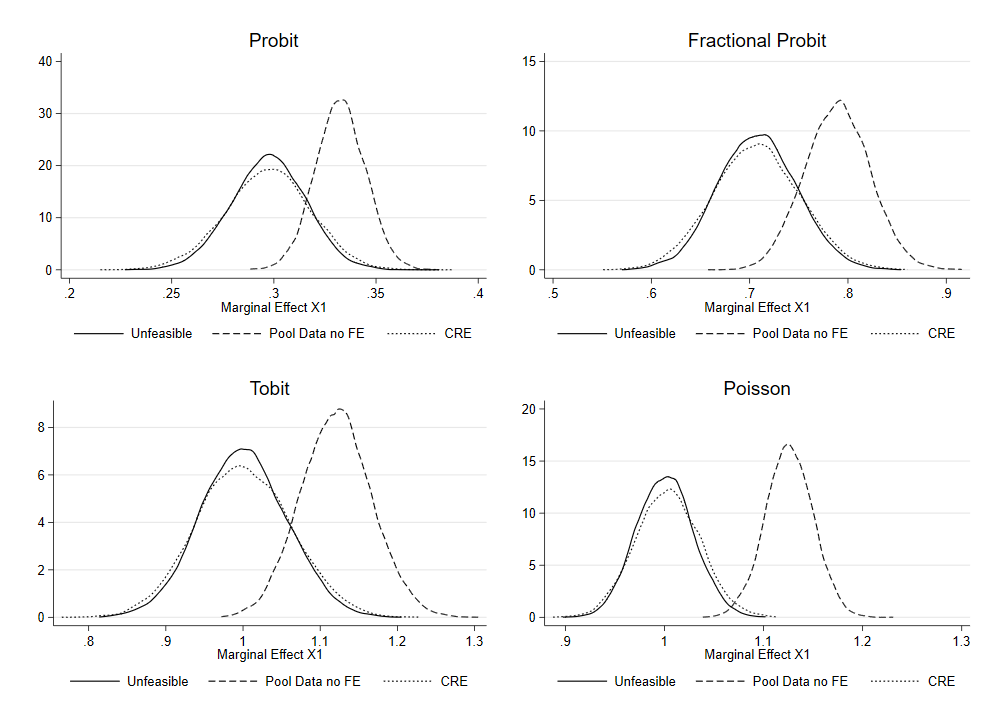
\includegraphics[keepaspectratio]{sim_v2/fig1.png}}

}

\caption{\label{fig-cre}Estimated APE/Coefficient densities for
non-linear models}

\end{figure}%

As expected, the unfeasible estimator, controlling directly for the
unobserved effect \texttt{c1}, provides the benchmark estimates. Since
the unobserved effect \texttt{c1} is correlated with \texttt{x1} and
\texttt{x2} by construction, the pooled estimators (which ignore
\texttt{c1}) exhibit significant bias, as seen in both the density plots
and the summary table.

In contrast, the CRE approach, implemented using the \texttt{cre}
prefix, yields estimates whose distributions are centered close to the
benchmark estimates, indicating negligible bias. While the CRE estimates
show slightly higher variance compared to the unfeasible benchmark (as
reflected in slightly larger MAE in Table~\ref{tbl-cre}), they
effectively mitigate the bias caused by the omitted correlated fixed
effect. This demonstrates the utility of the CRE method for obtaining
consistent estimates in nonlinear panel models where FE is not viable
and RE assumptions are violated.

\begin{longtable}[]{@{}
  >{\raggedright\arraybackslash}p{(\linewidth - 8\tabcolsep) * \real{0.2000}}
  >{\centering\arraybackslash}p{(\linewidth - 8\tabcolsep) * \real{0.2000}}
  >{\centering\arraybackslash}p{(\linewidth - 8\tabcolsep) * \real{0.2000}}
  >{\centering\arraybackslash}p{(\linewidth - 8\tabcolsep) * \real{0.2000}}
  >{\centering\arraybackslash}p{(\linewidth - 8\tabcolsep) * \real{0.2000}}@{}}
\caption{Bias and MAE for the estimated APE/Coefficients for non-linear
models (Coefficients for \texttt{x1})}\label{tbl-cre}\tabularnewline
\toprule\noalign{}
\begin{minipage}[b]{\linewidth}\raggedright
\end{minipage} & \begin{minipage}[b]{\linewidth}\centering
Probit
\end{minipage} & \begin{minipage}[b]{\linewidth}\centering
FProbit
\end{minipage} & \begin{minipage}[b]{\linewidth}\centering
Tobit
\end{minipage} & \begin{minipage}[b]{\linewidth}\centering
Poisson
\end{minipage} \\
\midrule\noalign{}
\endfirsthead
\toprule\noalign{}
\begin{minipage}[b]{\linewidth}\raggedright
\end{minipage} & \begin{minipage}[b]{\linewidth}\centering
Probit
\end{minipage} & \begin{minipage}[b]{\linewidth}\centering
FProbit
\end{minipage} & \begin{minipage}[b]{\linewidth}\centering
Tobit
\end{minipage} & \begin{minipage}[b]{\linewidth}\centering
Poisson
\end{minipage} \\
\midrule\noalign{}
\endhead
\bottomrule\noalign{}
\endlastfoot
True:Bias & 0.000 & -0.000 & -0.000 & -0.000 \\
True:MAE & 0.015 & 0.032 & 0.045 & 0.023 \\
Pool:Bias & 0.035 & 0.081 & 0.120 & 0.125 \\
Pool:MAE & 0.035 & 0.081 & 0.120 & 0.125 \\
CRE:Bias & -0.000 & -0.001 & 0.000 & 0.003 \\
CRE:MAE & 0.016 & 0.035 & 0.049 & 0.026 \\
\emph{N} & 10000 & 10000 & 10000 & 10000 \\
\end{longtable}

In the appendix, we extend the simulation to a more complex setting with
two unobserved fixed effects, which further illustrates the use of the
CRE approach in handling unbalanced panels and multiple dimensions of
unobserved heterogeneity. As mentioned before, however, when multiple
fixed effects are used, statistical inference remains challenging, and
the results should be interpreted with caution.

\section{Conclusion}\label{sec-6}

This paper introduced \texttt{cre}, a versatile Stata prefix command
designed to simplify the estimation of Correlated Random Effects (CRE)
models based on the \citet{mundlak1978pooling} specification. The CRE
approach provides a valuable bridge between standard Fixed Effects and
Random Effects models, offering several advantages: it allows for the
estimation of time-invariant variable effects (unlike FE) while
providing consistent estimates for time-varying coefficients even when
the strict RE exogeneity assumption fails (matching FE estimates in
linear models).

The primary contribution of the \texttt{cre} command lies in its
flexibility and ease of use. As a prefix command, it can be applied to a
wide array of standard Stata estimation commands, including user-written
ones. It automatically handles the generation of individual means for
time-varying covariates, supports both balanced and unbalanced panels,
and integrates seamlessly with factor variables and post-estimation
tools like \texttt{margins} for calculating Average Partial Effects,
which is particularly crucial for interpreting nonlinear models.

While \texttt{cre} offers a significant simplification for estimating
static, and potentially dynamic, CRE models, it does not address dynamic
auto-regressive panel models. The inclusion of lagged dependent
variables introduces further econometric challenges (e.g., the initial
conditions problem) that require specialized estimators beyond the scope
of this command.

In summary, the \texttt{cre} command provides applied researchers with a
user-friendly and powerful tool for leveraging the benefits of the
Correlated Random Effects approach in Stata, making it easier to
estimate models that account for unobserved heterogeneity while
retaining the ability to analyze the effects of time-invariant
characteristics, especially in nonlinear settings.

\section{Acknowledgments}\label{acknowledgments}

Thanks to Aashima Sinha for her help in the preparation and providing
feedback for this paper, and Enrique Pinzon for his encouragement on
pushing this project forward. I am also grateful to the Editor and an
anonymous referee for their constructive comments on a previous version,
which significantly improved the focus and clarity of this paper.

\section{References}\label{references}

\renewcommand{\bibsection}{}
\bibliography{references.bib}

\newpage
\appendix

\section*{Appendix}\label{appendix}
\addcontentsline{toc}{section}{Appendix}

\subsection*{Empirical ilustration: extended
results}\label{sec-appendix1}
\addcontentsline{toc}{subsection}{Empirical ilustration: extended
results}

In Section~\ref{sec-4}, I presented the empirical application of the
\texttt{cre} command using the \texttt{nlswork.dta} dataset, using
default standard errors. In this appendix, I provide additional results
using robust and clustered standard errors, as well as results for
two-way fixed effects models.

As it can be seen in Table~\ref{tbl-app1}, once robust standard errors
are used, the results for the linear model are almost identical to the
benchmark FE model, in terms of coefficients and standard errors
(proxied by t-statistics).

\begin{table}[H]

\caption{\label{tbl-app1}Comparison of Linear Models: Robust/Clustered
Standard Errors}

\centering{

\begin{tabular}{l*{5}{c}cccccccccc}
\hline\hline&\multicolumn{3}{c}{}&\multicolumn{2}{c}{CRE}\\
 &xtreg FE&xtreg RE&xtreg CRE &xtreg RE& regress\\
\hline
main        &            &            &            &            &            \\
age         &       0.042&       0.047&       0.042&       0.042&       0.042\\
            &      (9.74)&     (11.47)&      (9.74)&      (9.74)&      (9.74)\\
c.age\#c.age &      -0.001&      -0.001&      -0.001&      -0.001&      -0.001\\
            &     (-6.89)&     (-8.57)&     (-6.89)&     (-6.89)&     (-6.89)\\
tenure      &       0.041&       0.048&       0.041&       0.041&       0.041\\
            &     (18.99)&     (23.19)&     (18.99)&     (18.99)&     (18.99)\\
c.tenure\#c.tenure&      -0.001&      -0.002&      -0.001&      -0.001&      -0.001\\
            &    (-10.23)&    (-11.94)&    (-10.23)&    (-10.23)&    (-10.23)\\
1.white     &       0.000&       0.090&       0.081&       0.081&       0.093\\
            &         (.)&      (7.79)&      (7.27)&      (7.27)&      (8.02)\\
1.south     &      -0.071&      -0.121&      -0.071&      -0.071&      -0.071\\
            &     (-4.08)&    (-11.56)&     (-4.08)&     (-4.08)&     (-4.08)\\
m1\_age      &            &            &            &       0.051&       0.076\\
            &            &            &            &      (4.38)&      (5.95)\\
m1\_c\_age\_c\_age&            &            &            &      -0.001&      -0.001\\
            &            &            &            &     (-4.47)&     (-5.94)\\
m1\_tenure   &            &            &            &       0.074&       0.067\\
            &            &            &            &     (11.10)&      (9.11)\\
m1\_c\_tenure\_c\_tenure&            &            &            &      -0.003&      -0.003\\
            &            &            &            &     (-6.09)&     (-5.01)\\
m1\_\_1\_south &            &            &            &      -0.105&      -0.111\\
            &            &            &            &     (-5.14)&     (-5.36)\\
\_cons      &       0.835&       0.715&      -0.031&       0.792&       0.769\\
            &     (13.34)&     (12.11)&     (-0.21)&     (12.51)&     (12.16)\\
\hline
xt\_means    &            &            &            &            &            \\
age         &            &            &       0.051&            &            \\
            &            &            &      (4.38)&            &            \\
c.age\#c.age &            &            &      -0.001&            &            \\
            &            &            &     (-4.47)&            &            \\
tenure      &            &            &       0.074&            &            \\
            &            &            &     (11.10)&            &            \\
c.tenure\#c.tenure&            &            &      -0.003&            &            \\
            &            &            &     (-6.09)&            &            \\
1.white     &            &            &       0.000&            &            \\
            &            &            &         (.)&            &            \\
1.south     &            &            &      -0.105&            &            \\
            &            &            &     (-5.14)&            &            \\
\hline
\(N\)       &       28093&       28093&       28093&       28093&       28093\\
\hline\hline
\multicolumn{6}{l}{\footnotesize \textit{t} statistics in parentheses}\\
\end{tabular}

}

\end{table}%

In Table~\ref{tbl-app2}, I present the results for a two-way fixed
effects model, using the \texttt{cre}, absorbing both \texttt{idcode}
and \texttt{year} as fixed effects. As benchmark I use the
\texttt{reghdfe} command for the linear model, and \texttt{ppmlhdfe} for
the Poisson model. Three things to notice:

\begin{enumerate}
\def\labelenumi{\arabic{enumi}.}
\tightlist
\item
  \texttt{cre} produces the same point estimates as \texttt{reghdfe},
  showing the potential of the command.
\item
  \texttt{cre} produces very similar point estimates to
  \texttt{ppmlhdfe}. This is similar to what we observed in the main
  text.
\item
  Standard errors are different, and no correction was applied for
  \texttt{cre} other than providing \texttt{robust} standard errors.
\end{enumerate}

\begin{table}[H]

\caption{\label{tbl-app2}Comparison of Linear Models: Two-way Fixed
Effects}

\centering{

\begin{tabular}{l*{4}{c}cccccccc}
\hline\hline
            &\multicolumn{1}{c}{reghdfe}&\multicolumn{1}{c}{ppmlhdfe}&\multicolumn{1}{c}{CRE regress}&\multicolumn{1}{c}{CRE poisson}\\
\hline
main        &            &            &            &            \\
age         &       0.067&       0.069&       0.067&       0.067\\
            &      (5.59)&      (3.24)&      (4.08)&      (2.38)\\
c.age\#c.age &      -0.001&      -0.001&      -0.001&      -0.001\\
            &    (-13.11)&     (-7.71)&    (-10.07)&     (-5.89)\\
tenure      &       0.041&       0.037&       0.041&       0.037\\
            &     (24.07)&     (13.66)&     (17.40)&      (9.96)\\
c.tenure\#c.tenure&      -0.001&      -0.002&      -0.001&      -0.002\\
            &    (-13.27)&     (-6.22)&     (-9.37)&     (-4.84)\\
1.white     &       0.000&       0.000&       0.092&       0.099\\
            &         (.)&         (.)&     (16.58)&     (11.97)\\
1.south     &      -0.070&      -0.090&      -0.070&      -0.099\\
            &     (-5.33)&     (-4.64)&     (-4.14)&     (-3.48)\\
m1\_age      &            &            &       0.068&       0.093\\
            &            &            &      (3.69)&      (2.94)\\
m2\_age      &            &            &      -0.131&      -0.174\\
            &            &            &     (-3.88)&     (-3.67)\\
m1\_c\_age\_c\_age&            &            &      -0.001&      -0.002\\
            &            &            &     (-7.27)&     (-6.54)\\
m2\_c\_age\_c\_age&            &            &       0.003&       0.003\\
            &            &            &      (3.98)&      (3.83)\\
m1\_tenure   &            &            &       0.068&       0.046\\
            &            &            &     (14.58)&      (3.69)\\
m2\_tenure   &            &            &       0.068&       0.149\\
            &            &            &      (3.09)&      (5.16)\\
m1\_c\_tenure\_c\_tenure&            &            &      -0.003&      -0.001\\
            &            &            &     (-8.04)&     (-0.96)\\
m2\_c\_tenure\_c\_tenure&            &            &      -0.010&      -0.013\\
            &            &            &     (-3.09)&     (-3.18)\\
m1\_\_1\_south &            &            &      -0.108&      -0.076\\
            &            &            &     (-6.04)&     (-2.49)\\
m2\_\_1\_south &            &            &       0.313&       0.065\\
            &            &            &      (0.54)&      (0.08)\\
\_cons      &       0.506&       0.581&       0.440&       0.455\\
            &      (1.52)&      (0.90)&      (0.96)&      (0.55)\\
\hline
\(N\)       &       27541&       27541&       28093&       28093\\
\hline\hline
\multicolumn{5}{l}{\footnotesize \textit{t} statistics in parentheses}\\
\end{tabular}

}

\end{table}%

\subsection*{Two-way Fixed Effects}\label{sec-appendix2}
\addcontentsline{toc}{subsection}{Two-way Fixed Effects}

In this appendix, I provide results for the two-way fixed effects model,
using the \texttt{cre} command with two variables in the \texttt{abs()}
option. The results are similar to those presented in the main text.

\begin{figure}[H]

\centering{

\pandocbounded{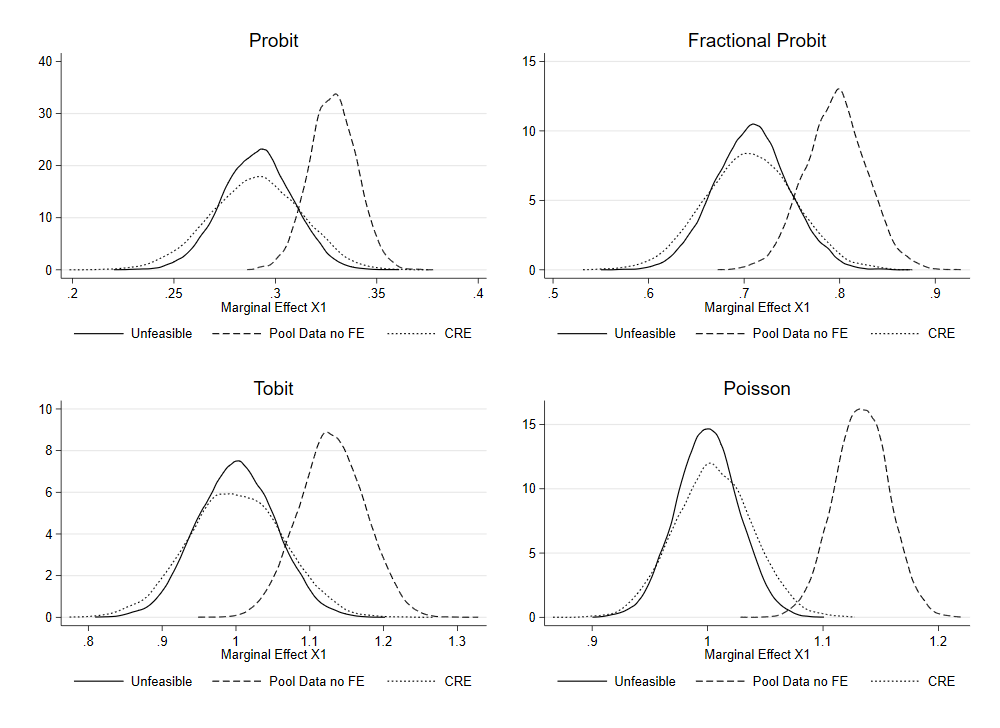
\includegraphics[keepaspectratio]{sim_v2/fig1_two.png}}

}

\caption{\label{fig-cre2}Estimated APE/Coefficient densities for
non-linear models: Two-way fixed effects}

\end{figure}%

\begin{longtable}[]{@{}
  >{\raggedright\arraybackslash}p{(\linewidth - 8\tabcolsep) * \real{0.2000}}
  >{\centering\arraybackslash}p{(\linewidth - 8\tabcolsep) * \real{0.2000}}
  >{\centering\arraybackslash}p{(\linewidth - 8\tabcolsep) * \real{0.2000}}
  >{\centering\arraybackslash}p{(\linewidth - 8\tabcolsep) * \real{0.2000}}
  >{\centering\arraybackslash}p{(\linewidth - 8\tabcolsep) * \real{0.2000}}@{}}
\caption{Bias and MAE for the estimated APE/Coefficients for non-linear
models TWFE: Coefficients for
\texttt{x1}}\label{tbl-cre2}\tabularnewline
\toprule\noalign{}
\begin{minipage}[b]{\linewidth}\raggedright
\end{minipage} & \begin{minipage}[b]{\linewidth}\centering
Probit
\end{minipage} & \begin{minipage}[b]{\linewidth}\centering
FProbit
\end{minipage} & \begin{minipage}[b]{\linewidth}\centering
Tobit
\end{minipage} & \begin{minipage}[b]{\linewidth}\centering
Poisson
\end{minipage} \\
\midrule\noalign{}
\endfirsthead
\toprule\noalign{}
\begin{minipage}[b]{\linewidth}\raggedright
\end{minipage} & \begin{minipage}[b]{\linewidth}\centering
Probit
\end{minipage} & \begin{minipage}[b]{\linewidth}\centering
FProbit
\end{minipage} & \begin{minipage}[b]{\linewidth}\centering
Tobit
\end{minipage} & \begin{minipage}[b]{\linewidth}\centering
Poisson
\end{minipage} \\
\midrule\noalign{}
\endhead
\bottomrule\noalign{}
\endlastfoot
True:Bias & -0.000 & 0.000 & 0.000 & -0.000 \\
True:MAE & 0.014 & 0.031 & 0.042 & 0.022 \\
Pool:Bias & 0.037 & 0.088 & 0.130 & 0.134 \\
Pool:MAE & 0.037 & 0.088 & 0.130 & 0.134 \\
CRE:Bias & -0.001 & -0.002 & -0.001 & 0.006 \\
CRE:MAE & 0.018 & 0.038 & 0.051 & 0.027 \\
\emph{N} & 10000 & 10000 & 10000 & 10000 \\
\end{longtable}

\clearpage

\bibliographystyle{sj}


\begin{aboutauthors}

Fernando Rios-Avila is an applied econometrician with passion for
econometrics and programming. His research interests include applied
econometrics, labor economics, and poverty and inequality. He has
contributed many commands to Statistical Software Components and written
articles for the Stata Journal.

\end{aboutauthors}

\end{document}
